\documentclass[a4paper,12pt]{article}
\usepackage{xcolor}
\usepackage{hyperref}
\usepackage{siunitx}
\usepackage{array}
\usepackage{tikz}
\usepackage{float} 
\usepackage{graphicx}
\usepackage{subcaption}
\usepackage{caption}


% Define link color for TOC
\hypersetup{
    colorlinks=true,
    linkcolor=blue,
    urlcolor=blue,
}

\begin{document}

% Title Page
\title{\textbf{Lab Report-8}\\Entry counter system using Up-Down Counter}
\author{Sai Akshita-EE24BTECH11054\\Sai Akhila-EE24BTECH11055}
\date{\today}
\maketitle

% Table of Contents with Blue Links
{\hypersetup{linkcolor=blue}
\tableofcontents}

\newpage

% Sections
\section{Objective}
To design and implement a digital up/down counter that displays the number of people currently
in the mess during peak lunch hours.

\section{Components Required}
\begin{itemize}
    \item 7-Segment Display (2-digit, Common Anode are used)
    \item Push Buttons (for simulation purposes if sensors are unavailable)
    \item Power Supply (5V DC for microcontroller and display)
    \item Breadboards and Jumper Wires
    \item Resistors ($\SI{1}{k\ohm}, \SI{100}{\ohm}$ for display connections)
    \item 2x 7447 Decoder
    \item 4x IC 7476(8-JK Flip Flops)
    \item IC 7432 for OR Gate (as required)
    \item IC 7408 for AND Gate (as required)
    \item IC 7404 for inverting gate (as required)
    \item IC 7486 for XOR gate (combining with not for XNOR)
    \item IC 7411 for 3-input AND gate (as required)
    \item IC 7421 for 4-input AND gate (as required)
    \item IC 7420 for 4-input NAND gate (as required)
\end{itemize}


\section{Circuit network Connections}

\subsection{Sketch of the Core-counting circuit}
This consists of Incrementing/Decrementing circuit, clock-pulse generating circuit, and sub-circuit consisting of T-flipflops which compute binary output of counter.
\begin{figure}[H]
    \centering
    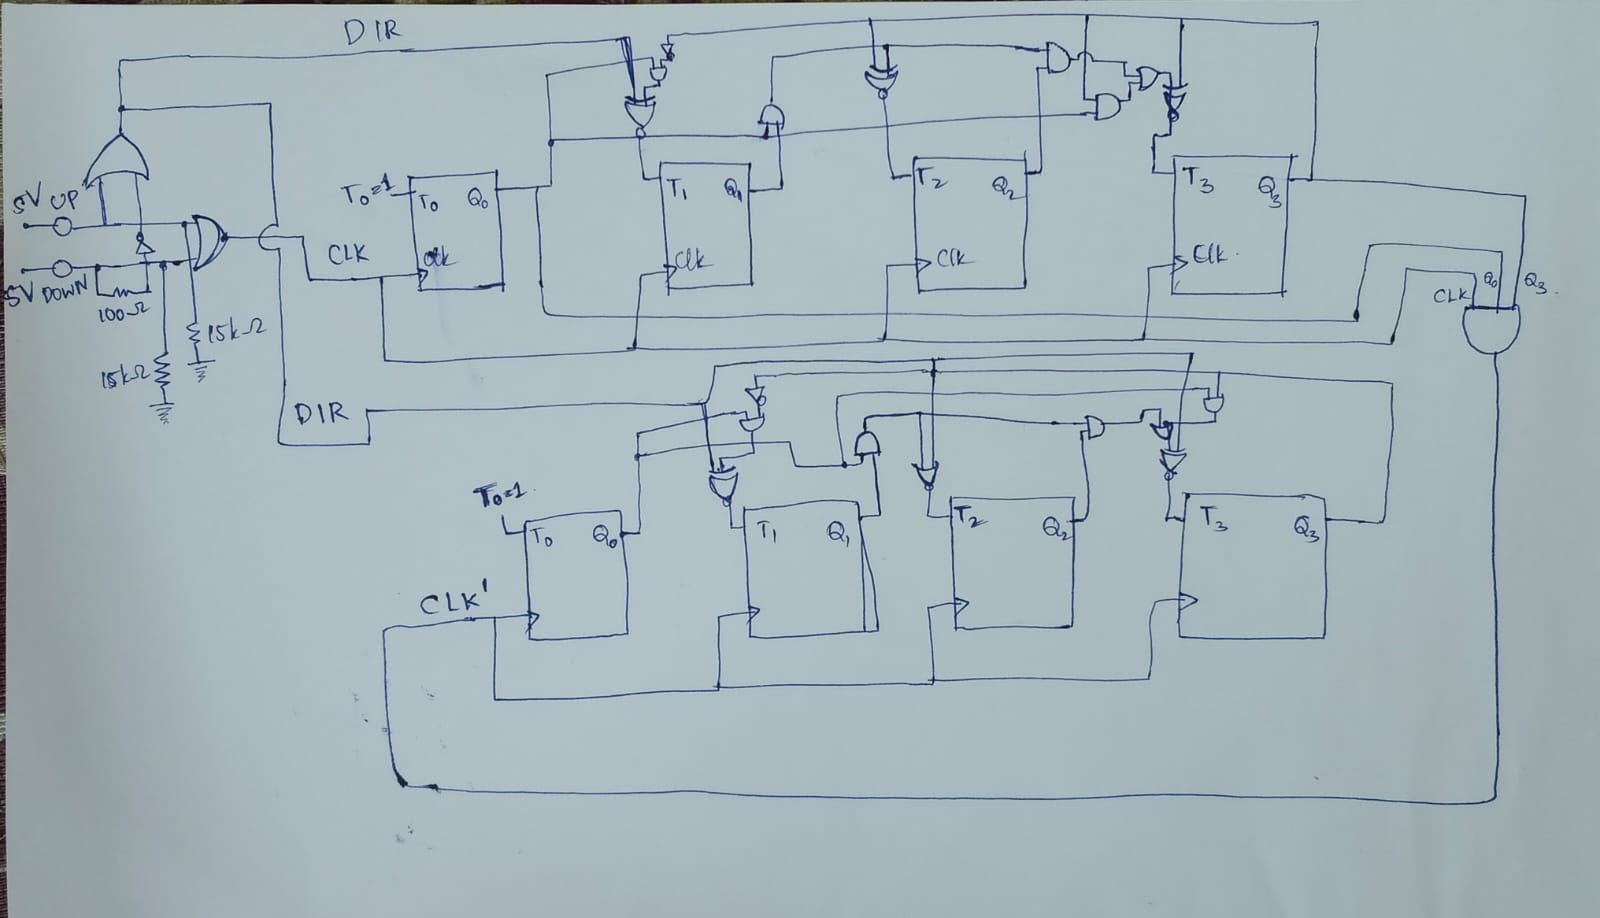
\includegraphics[width=0.5\textwidth]{ckt.png} % Replace with your image file
    \caption{Binary Core-counting circuit}
    \label{fig:my_label}
\end{figure}

\subsection{Incrementing/Decrementing circuit and clock-pulse generating circuit}
To navigate the incrementation or decrementation in count, the following circuit is built.

\begin{figure}[h!]
    \centering
    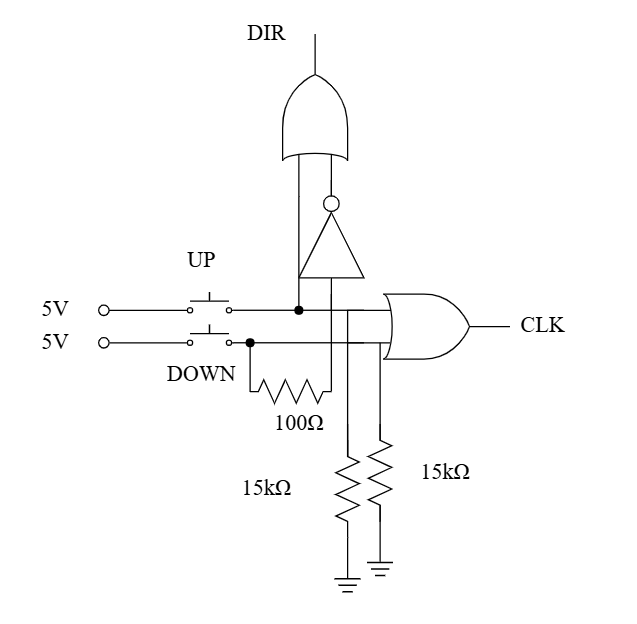
\includegraphics[width=\textwidth]{navi.png}
    \caption{clock-pulse generation circuit}
    \label{fig:image_label}
\end{figure}




\subsection{JK flip-flop connections for units digit}
\subsubsection{1st IC 7476(for bits $Q_0$ and $Q_1$)}
\begin{table}[H]
    \centering
    \renewcommand{\arraystretch}{1.3} % Adjust row height for better readability
    \begin{tabular}{|c|l|}
        \hline
        \textbf{Pin} & \textbf{Description} \\ 
        \hline
        1  & Clock for 1st flip-flop \\ 
        2  & $\overline{\text{PRESET}} = 1$ (For 1st flip-flop) \\ 
        3  & $\overline{\text{CLEAR}} = 1$ (For 1st flip-flop) \\ 
        4  & $J_0 = 1$ (should be connected to 5V) \\ 
        5  & Vcc = 5V \\ 
        6  & Clock for 2nd flip-flop \\ 
        7  & $\overline{\text{PRESET}} = 1$ (For 2nd flip-flop) \\ 
        8  & $\overline{\text{CLEAR}} = 1$ (For 2nd flip-flop) \\ 
        9  & $J_1 = Q_0.\overline{Q_3}.DIR+\overline{Q_0.\overline{Q_3}}.\overline{DIR}$ \\ 
        10 & $\overline{Q_1}$ \\ 
        11 & $Q_1$ \\ 
        12 & $K_1 = Q_0.\overline{Q_3}.DIR+\overline{Q_0.\overline{Q_3}}.\overline{DIR}$ \\ 
        13 & Ground (0V) \\ 
        14 & $\overline{Q_0}$ \\ 
        15 & $Q_0$ \\ 
        16 & $K_0 = 1$ (should be connected to 5V) \\ 
        \hline
    \end{tabular}
    \caption{Pin Configuration Table}
    \label{tab:pin_config_1}
\end{table}
\subsubsection{2nd IC 7476(for bits $Q_2$ and $Q_3$)}
\begin{table}[H]
    \centering
    \renewcommand{\arraystretch}{1.3} % Adjust row height for better readability
    \begin{tabular}{|c|l|}
        \hline
        \textbf{Pin} & \textbf{Description} \\ 
        \hline
        1  & Clock for 3rd flip-flop \\ 
        2  & $\overline{\text{PRESET}} = 1$ (For 3rd flip-flop) \\ 
        3  & $\overline{\text{CLEAR}} = 1$ (For 3rd flip-flop) \\ 
        4  & $J_2 = Q_0.Q_1.DIR+\overline{Q_0.Q_1}.\overline{DIR}$ \\ 
        5  & Vcc = 5V \\ 
        6  & Clock for 4th flip-flop \\ 
        7  & $\overline{\text{PRESET}} = 1$ (For 4th flip-flop) \\ 
        8  & $\overline{\text{CLEAR}} = 1$ (For 4th flip-flop) \\ 
        9  & $J_3 = (Q_0.Q_1.Q_2+Q_0.Q_3).DIR+\overline{(Q_0.Q_1.Q_2+Q_0.Q_3)}.\overline{DIR}$ \\ 
        10 & $\overline{Q_1}$ \\ 
        11 & $Q_3$ \\ 
        12 & $K_3 = (Q_0.Q_1.Q_2+Q_0.Q_3).DIR+\overline{(Q_0.Q_1.Q_2+Q_0.Q_3)}.\overline{DIR}$ \\ 
        13 & Ground (0V) \\ 
        14 & $\overline{Q_2}$ \\ 
        15 & $Q_2$ \\ 
        16 & $K_2 = Q_0.Q_1.DIR+\overline{Q_0.Q_1}.\overline{DIR}$ \\ 
        \hline
    \end{tabular}
    \caption{Pin Configuration Table}
    \label{tab:pin_config}
\end{table}

\subsection{JK flip-flop connections for tens digit}
\subsubsection{1st IC 7476(for bits $Q_0$ and $Q_1$)}
\begin{table}[H]
    \centering
    \renewcommand{\arraystretch}{1.3} % Adjust row height for better readability
    \begin{tabular}{|c|l|}
        \hline
        \textbf{Pin} & \textbf{Description} \\ 
        \hline
        1  & Clock for 1st flip-flop (From $Q_0.Q_3.CLK$) \\ 
        2  & $\overline{\text{PRESET}} = 1$ (For 1st flip-flop) \\ 
        3  & $\overline{\text{CLEAR}} = 1$ (For 1st flip-flop) \\ 
        4  & $J_0 = 1$ (should be connected to 5V) \\ 
        5  & Vcc = 5V \\ 
        6  & Clock for 2nd flip-flop (From $Q_0.Q_3.CLK$)\\ 
        7  & $\overline{\text{PRESET}} = 1$ (For 2nd flip-flop) \\ 
        8  & $\overline{\text{CLEAR}} = 1$ (For 2nd flip-flop) \\ 
        9  & $J_1 = Q_0.\overline{Q_3}.DIR+\overline{Q_0.\overline{Q_3}}.\overline{DIR}$ \\ 
        10 & $\overline{Q_1}$ \\ 
        11 & $Q_1$ \\ 
        12 & $K_1 = Q_0.\overline{Q_3}.DIR+\overline{Q_0.\overline{Q_3}}.\overline{DIR}$ \\ 
        13 & Ground (0V) \\ 
        14 & $\overline{Q_0}$ \\ 
        15 & $Q_0$ \\ 
        16 & $K_0 = 1$ (should be connected to 5V) \\ 
        \hline
    \end{tabular}
    \caption{Pin Configuration Table}
    \label{tab:pin_config_1}
\end{table}
\subsubsection{2nd IC 7476(for bits $Q_2$ and $Q_3$)}
\begin{table}[H]
    \centering
    \renewcommand{\arraystretch}{1.3} % Adjust row height for better readability
    \begin{tabular}{|c|l|}
        \hline
        \textbf{Pin} & \textbf{Description} \\ 
        \hline
        1  & Clock for 3rd flip-flop (From $Q_0.Q_3.CLK$)\\ 
        2  & $\overline{\text{PRESET}} = 1$ (For 3rd flip-flop) \\ 
        3  & $\overline{\text{CLEAR}} = 1$ (For 3rd flip-flop) \\ 
        4  & $J_2 = Q_0.Q_1.DIR+\overline{Q_0.Q_1}.\overline{DIR}$ \\ 
        5  & Vcc = 5V \\ 
        6  & Clock for 4th flip-flop (From $Q_0.Q_3.CLK$)\\ 
        7  & $\overline{\text{PRESET}} = 1$ (For 4th flip-flop) \\ 
        8  & $\overline{\text{CLEAR}} = 1$ (For 4th flip-flop) \\ 
        9  & $J_3 = (Q_0.Q_1.Q_2+Q_0.Q_3).DIR+\overline{(Q_0.Q_1.Q_2+Q_0.Q_3)}.\overline{DIR}$ \\ 
        10 & $\overline{Q_1}$ \\ 
        11 & $Q_3$ \\ 
        12 & $K_3 = (Q_0.Q_1.Q_2+Q_0.Q_3).DIR+\overline{(Q_0.Q_1.Q_2+Q_0.Q_3)}.\overline{DIR}$ \\ 
        13 & Ground (0V) \\ 
        14 & $\overline{Q_2}$ \\ 
        15 & $Q_2$ \\ 
        16 & $K_2 = Q_0.Q_1.DIR+\overline{Q_0.Q_1}.\overline{DIR}$ \\ 
        \hline
    \end{tabular}
    \caption{Pin Configuration Table}
    \label{tab:pin_config}
\end{table}
 

\subsection{Flip Flops to Decoder}
\begin{table}[H]
    \centering
    \renewcommand{\arraystretch}{1.3}
    \begin{tabular}{|c|c|}
        \hline
        \textbf{Output bit} & \textbf{7447 Pin} \\
        \hline
        $Q_0$ & A \\
        $Q_1$ & B \\
        $Q_2$ & C \\
        $Q_3$ & D \\
        \hline
    \end{tabular}
    \caption{Connections from output bits (IC 7476) to 7447 Decoder}
    \label{tab:7447_connections}
\end{table}
\begin{itemize}
    \item \textbf{The output bits $Q_0$ to $Q_3$ represent the BCD of a number.}
    \item \textbf{To represet the BCD equivalent of a number on Seven-Segment display, decoder is used.}
    \item \textbf{We use 2 decoders in the entire circuit (one for a digit) to convert BCD to seven segment display.}
\end{itemize}


\subsection{Decoder to seven-segment display}
\begin{table}[H]
    \centering
    \renewcommand{\arraystretch}{1.3}
    \begin{tabular}{|c|c|}
        \hline
        \textbf{7447 Pin} & \textbf{Seven-Segment Display Segment} \\
        \hline
        $\overline{a}$ & a \\
        $\overline{b}$ & b \\
        $\overline{c}$ & c \\
        $\overline{d}$ & d \\
        $\overline{e}$ & e \\
        $\overline{f}$ & f \\
        $\overline{g}$ & g \\
        \hline
    \end{tabular}
    \caption{Connections from 7447 Decoder to Seven-Segment Display}
    \label{tab:7447_connections}
\end{table}


\section{Logic}
\subsection{Excitation Table for JK Flip-Flop}
\begin{table}[H]
    \centering
    \renewcommand{\arraystretch}{1.3}
    \begin{tabular}{|c|c||c|c|}
        \hline
        \textbf{$Q_n$} & \textbf{$Q_{n+1}$} & \textbf{J} & \textbf{K} \\
        \hline
        0 & 0 & 0 & X \\
        0 & 1 & 1 & X \\
        1 & 0 & X & 1 \\
        1 & 1 & X & 0 \\
        \hline
    \end{tabular}
    \caption{Excitation Table for JK Flip-Flop}
    \label{tab:jk_excitation}
\end{table}

\subsection{Excitation Table for T Flip-Flop}
\begin{table}[h!]
\centering
\caption{Excitation Table for T Flip-Flop}
\begin{tabular}{|c|c|c|}
\hline
\textbf{Present State ($Q_n$)} & \textbf{Next State ($Q_{n+1}$)} & \textbf{T Input} \\
\hline
0 & 0 & 0 \\
0 & 1 & 1 \\
1 & 0 & 1 \\
1 & 1 & 0 \\
\hline
\end{tabular}
\end{table}


\subsection{Truth Table for incrementing logic}
\begin{table}[H]
    \centering
    \renewcommand{\arraystretch}{1.3}
    \begin{tabular}{|c|c|c|c|c|c|c|c|c|c|c|c|c|c|c|c|}
        \hline
        \textbf{Q3} & \textbf{Q2} & \textbf{Q1} & \textbf{Q0} & \textbf{J3} & \textbf{K3} & \textbf{J2} & \textbf{K2} & \textbf{J1} & \textbf{K1} & \textbf{J0} & \textbf{K0} & \textbf{NS3} & \textbf{NS2} & \textbf{NS1} & \textbf{NS0} \\
        \hline
       0 & 0 & 0 & 0 &0 &X &0 & X& 0& X& 1& X& 0 & 0 & 0 & 1 \\
        0 & 0 & 0 & 1 &0 &X &0 &X &1 &X &X & 1& 0 & 0 & 1 & 0 \\
        0 & 0 & 1 & 0 & 0& X& 0& X& X& 0& 1& X&  0 & 0 & 1 & 1 \\
        0 & 0 & 1 & 1 &0 &X &1 &X &X &1 &X &1 & 0 & 1 & 0 & 0 \\
        0 & 1 & 0 & 0 &0 &X &X &0 &0 &X &1 &X & 0 & 1 & 0 & 1 \\
        0 & 1 & 0 & 1 & 0&X &X &0 &1 &X &X &1 &  0 & 1 & 1 & 0 \\
        0 & 1 & 1 & 0 & 0& X& X& 0& X& 0& 1& X&  0 & 1 & 1 & 1 \\
        0 & 1 & 1 & 1 & 1& X&X &1 &X &1 &X &1 & 1 & 0 & 0 & 0 \\
        1 & 0 & 0 & 0 &X &0 &0 &X &0 &X &1 &X & 1 & 0 & 0 & 1 \\
        1 & 0 & 0 & 1 &X & 1&0 &X & 0&X &X &1& 0 & 0 & 0 & 0 \\
        \hline
        1 & 0 & 1 & 0 & X& X& X&X &X & X&X &X & X & X & X & X \\
        1 & 0 & 1 & 1 & X& X&X & X&X & X&X & X& X & X & X & X \\
        1 & 1 & 0 & 0 & X& X&X &X &X &X &X &X & X & X & X & X \\
        1 & 1 & 0 & 1 & X& X& X& X& X& X& X& X& X & X & X & X \\
        1 & 1 & 1 & 0 & X&X &X & X& X& X& X& X& X & X & X & X \\
        1 & 1 & 1 & 1 & X& X& X& X& X& X& X& X& X & X & X & X \\
        \hline
    \end{tabular}
    \caption{Truth Table for Incrementation}
    \label{tab:truth_table}
\end{table}

\newpage
\subsection{K-maps for J and K of each flip-flop(Incrementation)}

\begin{figure}[H]
    \centering

    % First row
    \begin{subfigure}[b]{0.45\textwidth}
        \centering
        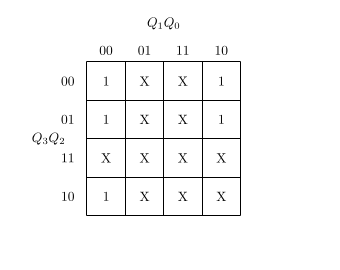
\includegraphics[width=\linewidth]{inc/ij0.png}
        \caption{$J_0=1$}
    \end{subfigure}
    \hfill
    \begin{subfigure}[b]{0.45\textwidth}
        \centering
        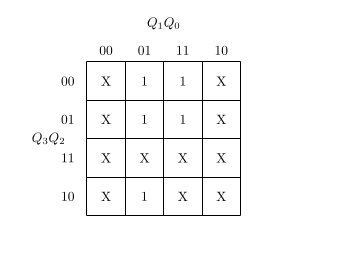
\includegraphics[width=\linewidth]{inc/ik0.png}
        \caption{$K_0=1$}
    \end{subfigure}

    \vspace{0.5cm}

    % Second row
    \begin{subfigure}[b]{0.45\textwidth}
        \centering
        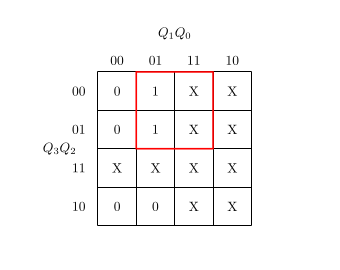
\includegraphics[width=\linewidth]{inc/ij1.png}
        \caption{$J_1=Q_0.\overline{Q_3}$}
    \end{subfigure}
    \hfill
    \begin{subfigure}[b]{0.45\textwidth}
        \centering
        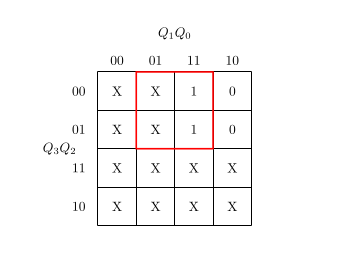
\includegraphics[width=\linewidth]{inc/ik1.png}
        \caption{$K_1=Q_0.\overline{Q_3}$}
    \end{subfigure}

    \caption{JK values of 1st IC7476}
\end{figure}

\newpage
\begin{figure}[H]
    \centering

    % First row
    \begin{subfigure}[b]{0.45\textwidth}
        \centering
        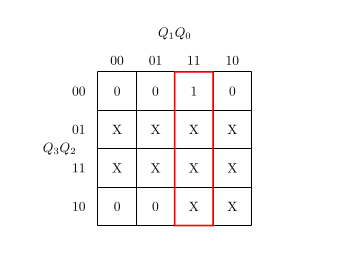
\includegraphics[width=\linewidth]{inc/ij2.png}
        \caption{$J_2=Q_0.Q_1$}
    \end{subfigure}
    \hfill
    \begin{subfigure}[b]{0.45\textwidth}
        \centering
        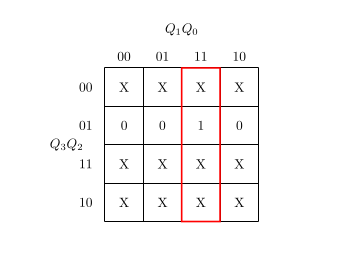
\includegraphics[width=\linewidth]{inc/ik2.png}
        \caption{$K_2=Q_0.Q_1$}
    \end{subfigure}

    \vspace{0.5cm}

    % Second row
    \begin{subfigure}[b]{0.45\textwidth}
        \centering
        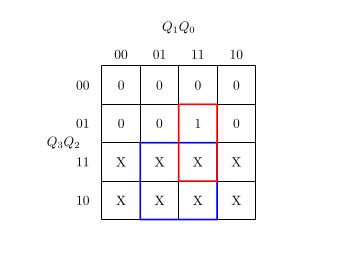
\includegraphics[width=\linewidth]{inc/ij3.png}
        \caption{$J_3=(Q_0.Q_1.Q_2)+(Q_0.Q_3)$}
    \end{subfigure}
    \hfill
    \begin{subfigure}[b]{0.45\textwidth}
        \centering
        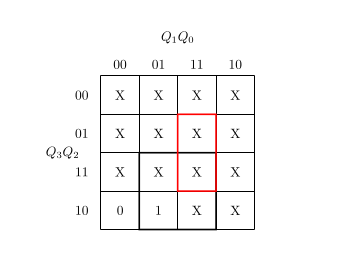
\includegraphics[width=\linewidth]{inc/ik3.png}
        \caption{$K_3=(Q_0.Q_1.Q_2)+(Q_0.Q_3)$}
    \end{subfigure}

    \caption{JK values of 2nd IC7476}
\end{figure}

\newpage






\subsection{Truth table for Decrementing Logic}
\begin{table}[H]
    \centering
    \renewcommand{\arraystretch}{1.3}
    \begin{tabular}{|c|c|c|c|c|c|c|c|c|c|c|c|c|c|c|c|}
        \hline
        \textbf{Q3} & \textbf{Q2} & \textbf{Q1} & \textbf{Q0} & \textbf{J3} & \textbf{K3} & \textbf{J2} & \textbf{K2} & \textbf{J1} & \textbf{K1} & \textbf{J0} & \textbf{K0} & \textbf{NS3} & \textbf{NS2} & \textbf{NS1} & \textbf{NS0} \\
        \hline
        1 & 1 & 1 & 1 & X&X & X&X &X &X &X&X& X&X & X&X \\
        1 & 1 & 1 & 0 & X& X& X& X& X& X& X&X&X&X & X&X \\
        1 & 1 & 0 & 1 & X&X & X&X & X&X &X&X& X&X & X&X\\
        1 & 1 & 0 & 0 & X&X &X & X& X& X& X&X&X&X & X&X \\
        1 & 0 & 1 & 1 & X&X & X&X &X & X&X&X& X&X & X&X \\
        1 & 0 & 1 & 0 & X&X & X& X& X& X&X&X& X&X & X&X\\
        \hline
        1 & 0 & 0 & 1 &X &0 &0 &X &0 &X &X &1 & 1 & 0 & 0 & 0 \\
        1 & 0 & 0 & 0 &X &1 &1 &X &1 &X &1 &X & 0 & 1 & 1 & 1 \\
        0 & 1 & 1 & 1 &0 &X &X &0 &X &0 &X &1 & 0 & 1 & 1 & 0 \\
        0 & 1 & 1 & 0 &0 &X &X &0 &X &1 &1 &X & 0 & 1 & 0 & 1 \\
        0 & 1 & 0 & 1 &0 &X &X &0 &0 &X &X &1 & 0 & 1 & 0 & 0 \\
        0 & 1 & 0 & 0 &0 &X &X &1 &1 &X &1 &X & 0 & 0 & 1 & 1 \\
        0 & 0 & 1 & 1 &0 &X &0 &X &X &0 &X &1 & 0 & 0 & 1 & 0 \\
        0 & 0 & 1 & 0 &0 &X &0 &X &X &1 &1 &X & 0 & 0 & 0 & 1 \\
        0 & 0 & 0 & 1 &0 &X &0 &X &0 &X &X &1 & 0 & 0 & 0 & 0 \\
        0 & 0 & 0 & 0 &1 &X &0 &X &0 &X &1 &X & 1 & 0 & 0 & 1 \\
        \hline
    \end{tabular}
    \caption{Truth Table for Decrementation}
    \label{tab:truth_table}
\end{table}
\newpage
\subsection{K-maps for J and K of each flipflop(Decrementation)}
\begin{figure}[H]
    \centering

    % First row
    \begin{subfigure}[b]{0.45\textwidth}
        \centering
        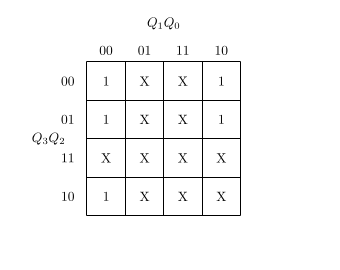
\includegraphics[width=\linewidth]{dec/dj0.png}
        \caption{$J_0=1$}
    \end{subfigure}
    \hfill
    \begin{subfigure}[b]{0.45\textwidth}
        \centering
        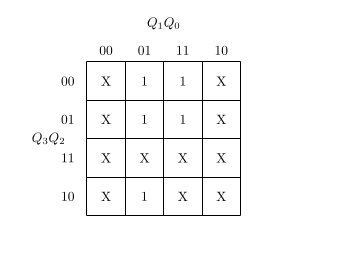
\includegraphics[width=\linewidth]{dec/dk0.png}
        \caption{$K_0=1$}
    \end{subfigure}

    \vspace{0.5cm}

    % Second row
    \begin{subfigure}[b]{0.45\textwidth}
        \centering
        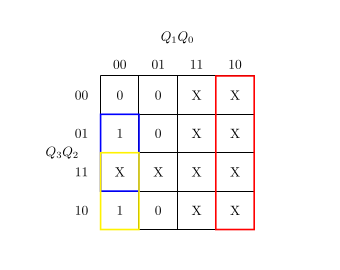
\includegraphics[width=\linewidth]{dec/dj1.png}
        \caption{$J_1=\overline{Q_0}Q_1+\overline{Q_0}\overline{Q_1}(Q_2+Q_3)$}
    \end{subfigure}
    \hfill
    \begin{subfigure}[b]{0.45\textwidth}
        \centering
        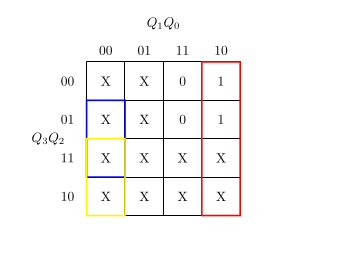
\includegraphics[width=\linewidth]{dec/dk1.png}
        \caption{$K_1=\overline{Q_0}Q_1+\overline{Q_0}\overline{Q_1}(Q_2+Q_3)$}
    \end{subfigure}

    \caption{JK values of 3rd IC7476}
\end{figure}
\newpage
\begin{figure}[H]
    \centering

    % First row
    \begin{subfigure}[b]{0.45\textwidth}
        \centering
        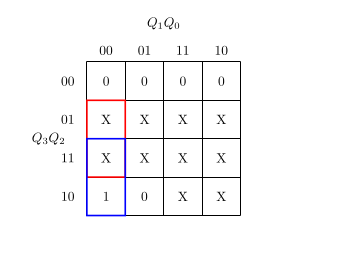
\includegraphics[width=\linewidth]{dec/dj2.png}
        \caption{$J_2=\overline{Q_0}\overline{Q_1}(Q_3+Q_2)$}
    \end{subfigure}
    \hfill
    \begin{subfigure}[b]{0.45\textwidth}
        \centering
        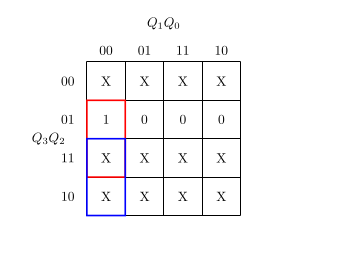
\includegraphics[width=\linewidth]{dec/dk2.png}
        \caption{$K_2=\overline{Q_0}\overline{Q_1}(Q_3+Q_2)$}
    \end{subfigure}

    \vspace{0.5cm}

    % Second row
    \begin{subfigure}[b]{0.45\textwidth}
        \centering
        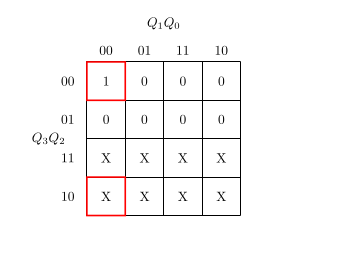
\includegraphics[width=\linewidth]{dec/dj3.png}
        \caption{$J_3=\overline{Q_0Q_1Q_2}$}
    \end{subfigure}
    \hfill
    \begin{subfigure}[b]{0.45\textwidth}
        \centering
        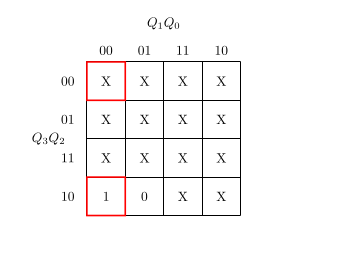
\includegraphics[width=\linewidth]{dec/dk3.png}
        \caption{$K_3=\overline{Q_0Q_1Q_2}$}
    \end{subfigure}

    \caption{JK values of 4th IC7476}
\end{figure}


\section{Working Principle of circuit}

\subsubsection{Working of DIR}
The \texttt{DIR} signal acts as a control input to decide the counting direction:
\begin{itemize}
    \item \textbf{DIR = 1 (High)}: The counter increments.
    \item \textbf{DIR = 0 (Low)}: The counter decrements.
\end{itemize}

\subsection{Implementation with Push Buttons}
Push buttons play a crucial role in manually controlling the \texttt{DIR} signal. The common configurations are:
\subsubsection{Two-Button Configuration}
Two push buttons can be used:
\begin{itemize}
    \item \textbf{Increment Button (UP)}: When pressed, it sets \texttt{DIR} = 1 and triggers a clock pulse. Pressing the UP button generates a pulse that signifies an increment.
    \item \texttt{DIR}=1, The output function is the boolean logic associated with \texttt{DIR}, results in enabling $J_1=K_1=Q_0.\overline{Q_3}$, and similar will happen for $J_2=K_2$ and $J_3=K_3$.
    \item \textbf{Decrement Button (DOWN)}: When pressed, it sets \texttt{DIR} = 0 and triggers a clock pulse. Pressing the DOWN button generates a pulse that signifies a decrement.
    \item \texttt{DIR}=0, The the output function is the boolean logic associated with \texttt{DIR}, results in enabling $J_1=K_1=\overline{Q_0}Q_1+\overline{Q_0}\overline{Q_1}(Q_2+Q_3)$, and similar will happen for $J_2=K_2$ and $J_3=K_3$.
\end{itemize}

\subsubsection{Single-Button Toggle Configuration}
A single push button can toggle the \texttt{DIR} state:
\begin{itemize}
    \item Pressing the button flips \texttt{DIR} from 0 to 1 (increment mode) and vice versa.
    \item A debounce circuit or software debouncing had been setup to ensure a stable transition.
\end{itemize}

\subsubsection{Role of Resistors}
\begin{itemize}
    \item The 100$\Omega$ resistor between push button of DOWN and NOT gate acts as a current-limiting resistor to prevent excessive current when the DOWN button is pressed.
    \item The 15k$\Omega$ pull-down resistors ensure the logic state of the gates remains LOW when no buttons are pressed, avoiding floating inputs.
\end{itemize}

\subsection{Working Principle of clock-pulse generation circuit and DIR}
\subsubsection{Working of clock pulse for units and tens digit}
\begin{itemize}
    \item For the flip flops contributing to units digit, the clock pulse is given directly from clock-pulse generator circuit, so as to increment/decrement the digit.
    \item For the flip flops contributing to tens digit, the clock signal is given by the \textbf{AND} of $Q_0$,$Q_3$, and the CLK generated by the clock-pulse generator circuit.
\end{itemize}

\subsubsection{Logic behind the CLOCK of tens digit}
\begin{itemize}
    \item \textbf{Incrementing:}When the units digit reaches 9 and the UP button is pushed, the tens digit has to increase by 1. The BCD equivalent of 9 is $1001$, which means the \textbf{AND} of $Q_0$,$Q_3$, and the CLK goes from 1 to 0,causing negative edge trigger and DIR becoming 1 results in incrementation of the tens digit.
    \item Since the 4-bits of units digit are synchronous, the units digit automatically resets to 0.
    \item \textbf{Decrementing:}When the units digit reach 0 and the DOWN button is pushed, the tens digit has to decrease by 1. The BCD equivalent of 9 is $1001$, which means the \textbf{AND} of $Q_0$,$Q_3$, and the CLK goes from 1 to 0,causing negative edge trigger and DIR becoming 0 results in decrementation of the tens digit.
    \item Since the 4-bits of units digit are synchronous, the units digit automatically resets to 9.
\end{itemize}


\subsection{T-Flip-flop sub circuit and Decoder and 7-segment setup}

\subsubsection{T-Flip-flop sub circuit for units digit}
\begin{itemize}
    \item Each flip-flop receives CLOCK from clock-pulse generator circuit.
    \item Since we are using T-flip-flops, for IC 7476, both J and K are given same logic.
    \item Each flip flop input requires corresponding logic, it it listed in logic section. The logic is provided using whatever ICs are required.
    \item The outputs $Q_0$ to $Q_3$ for each digit are generated by 4 flip-flops whose manual connections and logic are mentioned above.
\end{itemize}

\subsubsection{T-Flip-flop sub circuit for tens digit}
\begin{itemize}
    \item Each flip-flop receives CLOCK from the \textbf{AND} of $Q_0,Q_3$ and CLK generated from clock-pulse generator circuit.
    \item Since we are using T-flip-flops, for IC 7476, both J and K are given same logic.
    \item Each flip flop input requires corresponding logic, it it listed in logic section. The logic is provided using whatever ICs are required.
    \item The outputs $Q_0$ to $Q_3$ for each digit are generated by 4 flip-flops whose manual connections and logic are mentioned above.
\end{itemize}

\subsubsection{Decoder and 7-segment display}
\begin{itemize}
    \item The outputs $Q_0$ to $Q_3$ for each digit are generated by 4 flip-flops whose manual connections and logic are mentioned above.
    \item For each digit, each of $Q_0$ to $Q_3$ outputs are sent to IC 7447 decoder and from there, the corresponding number is displayed on seven-segment display.
\end{itemize}

\section{Conclusion}
Hence, we can implement a double digit partially synchronous counter using Boolean logic and T-Flip-Flops.

\end{document}

